%
% CSE Electronic Homework Template
% Last modified 8/23/2018 by Jeremy Buhler

\documentclass[11pt]{article}
\usepackage[left=0.7in,right=0.7in,top=1in,bottom=0.7in]{geometry}
\usepackage{fancyhdr} % for header
\usepackage{graphicx} % for figures
\usepackage{amsmath}  % for extended math markup
\usepackage{amssymb}
\usepackage[bookmarks=false]{hyperref} % for URL embedding
\usepackage[noend]{algpseudocode} % for pseudocode
\usepackage[plain]{algorithm} % float environment for algorithms

%%%%%%%%%%%%%%%%%%%%%%%%%%%%%%%%%%%%%%%%%%%%%%%%%%%%%%%%%%%%%%%%%%%%%%
% STUDENT: modify the following fields to reflect your
% name/ID, the current homework, and the current problem number

% Example: 
%\newcommand{\StudentName}{Jeremy Buhler}
%\newcommand{\StudentID{123456}

\newcommand{\StudentName}{Howard Wang}
\newcommand{\StudentID}{Analyzing Google Play Store Apps Data}
\newcommand{\HomeworkNumber}{Project Part 3}

%%%%%%%%%%%%%%%%%%%%%%%%%%%%%%%%%%%%%%%%%%%%%%%%%%%%%%%%%%%%%%%%%%%%%%%%
% You can pretty much leave the stuff up to the next line of %%'s alone.

% create header and footer for every page
\pagestyle{fancy}
\fancyhf{}
\lhead{\textbf{\StudentName}}
\chead{\textbf{\StudentID}}
\rhead{\textbf{\HomeworkNumber}}
\cfoot{\thepage}

% preferred pseudocode style
\algrenewcommand{\algorithmicprocedure}{}
\algrenewcommand{\algorithmicthen}{}

% ``do { ... } while (cond)''
\algdef{SE}[DOWHILE]{Do}{doWhile}{\algorithmicdo}[1]{\algorithmicwhile\ #1}%

% ``for (x in y ... z)''
\newcommand{\ForRange}[3]{\For{#1 \textbf{in} #2 \ \ldots \ #3}}

% these are common math formatting commands that aren't defined by default
\newcommand{\union}{\cup}
\newcommand{\isect}{\cap}
\newcommand{\ceil}[1]{\ensuremath \left\lceil #1 \right\rceil}
\newcommand{\floor}[1]{\ensuremath \left\lfloor #1 \right\rfloor}

%%%%%%%%%%%%%%%%%%%%%%%%%%%%%%%%%%%%%%%%%%%%%%%%%%%%%%%%%%%%%%%%%%%%%%
\usepackage[utf8]{inputenc}
\usepackage[english]{babel}
\setlength{\parindent}{0em}
\setlength{\parskip}{1em}
 \usepackage{pythonhighlight}
\usepackage{graphicx}
\graphicspath{ {./images/} }


\begin{document}
\underline{\textbf{Model 1: Random Forest}}\\ \\
\textbf{Business Problem}: \\
A business or individual would certainly want to predict how popular an app will be. One reasonable way to define that is based on the number of installs.  We can consider an app with over 1,000,000 downloads to be popular and those with downloads below that to be unpopular. We want to build a model to predict whether a new app will be a popular app.

\textbf{Analysis and Modeling}: \\
After cleaning the data, there were 8892 rows. 2566 apps had over 1,000,000 install or more, and 6326 apps had installs less than that. I set aside 20\% of the data for testing allocating around the same proportion of over and less than 1,000,000 install apps as the training set.

I did not apply standardization on the data for the random forest. Using the backward selection algorithm (from one of the homeworks), I decided to go with 5 features. However, deleting variables is not extremely necessary for tree algorithms.\\
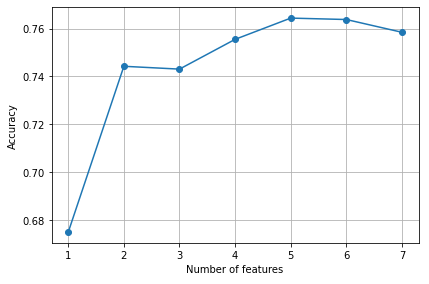
\includegraphics[scale=0.5]{vip1} \\

Random Forests are one of the most popular machine learning algorithms with good accuracy, robust to outliers, and less risk of overfitting. I used the data with the attributes Category, Rating, Price, Content Rating, Genres, and built a random forest model with the following parameters. \\ \\
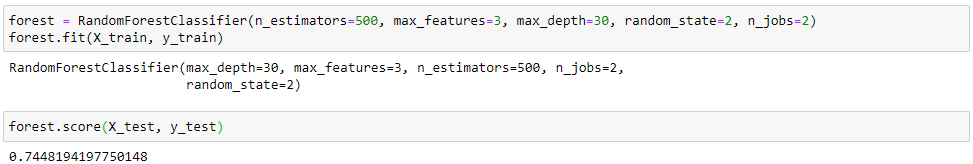
\includegraphics[scale=0.65]{model11} \\

Using the data with the features Category, Rating, Price, Content Rating, Genres, the random forest model achieved close to a 75\% accuracy, which is reasonable. Including the number of reviews in the model will dramatically increase the accuracy rate, however the number of reviews may not be known beforehand so I did not include it. Also, the confusion matrix can better illustrate the fit of the model. \\
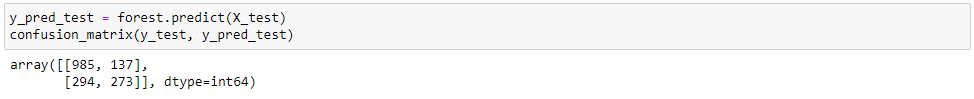
\includegraphics[scale=0.65]{confusion} \\ \\ \\

\underline{\textbf{Model 2: K-Nearest Neighbor Regression}}\\ \\
\textbf{Business Problem}: \\
An app developer may be interested in predicting the rating of the app. Better ratings will better reflect the app as well as the reputation of the developer or company. Apps with higher ratings could potentially attract more users. So it is importantly accurately predict the rating of an app. This is a regression problem.

\textbf{Analysis and Modeling}: \\
I applied a KNN algorithm to predicting the app ratings.  I standardized the data as KNN is sensitive to scaling. I decided to add all the features to the model. KNN only has 1 parameter that needs tuning, which is the K value. A guideline online is to use k to be around squareroot of N. After experimenting, K=60 worked well for this data set. A more accurate K can be determined from cross-validation, which I can explore in the next part of the project (testing). \\ \\ \\
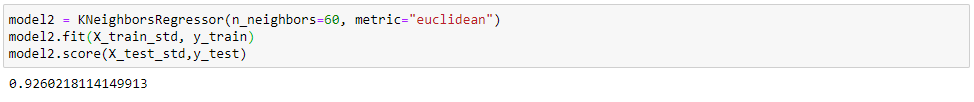
\includegraphics[scale=0.65]{KNN2} \\ 

We got a model with a R squared of 92.6\%, which is good. Which means 92.6\% of the variance in Rating is explained by the predictors. We can also get the MSE and RMSE of the model. And both numbers are fairly low. \\ 
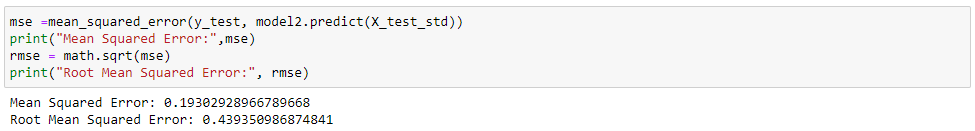
\includegraphics[scale=0.65]{rmse} \\  \\ \\ \\ \\ \\ \\ \\ \\ \\ \\ \\ \\ \\ \\ \\ \\ \\ \\ \\

\underline{\textbf{Model 3: K-Means Clustering (Unsupervised)}}\\ \\
\textbf{Business Problem}: \\
A business might be interested in identifying apps where people have strong feelings about or apps that people don't have much to say about. In our scenario, we would define that as apps with high number of reviews but high number of downloads or apps with high number of downloads but low number of reviews. Apps with high number of reviews, but low downloads could also signal abnormalities, such as a lot of people posting review about a technical problem with the app. Information like these will be helpful for companies. So we are looking for clusters.  \\ 

\textbf{Analysis and Modeling}: \\
K-means is an unsupervised algorithm that can identify clusters in a data set. I applied this algorithm to our data set with Reviews and Installs as features. For K-means it's important the features be the same scale. I standardized the two features using the standard scaler. We can pick K, the number of clusters, using the elbow method. From this graph, I decided to pick K=5. \\ \\
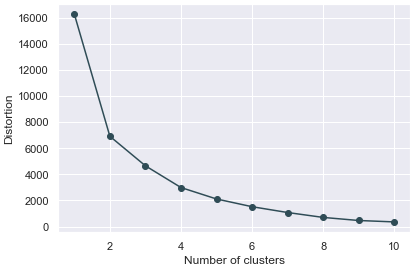
\includegraphics[scale=0.65]{elbow} \\ 
The initial plot of reviews and installs after standardizing looks like. \\ \\
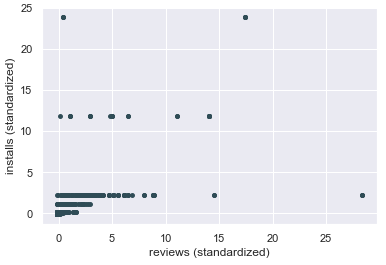
\includegraphics[scale=0.65]{kmeans1} \\ 
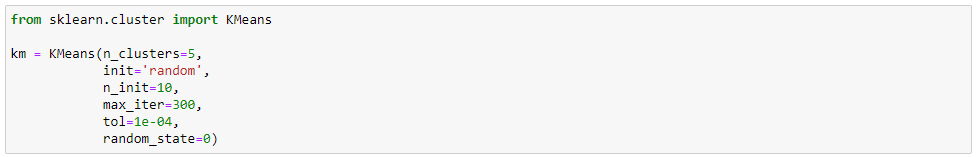
\includegraphics[scale=0.65]{kmodel} \\ 
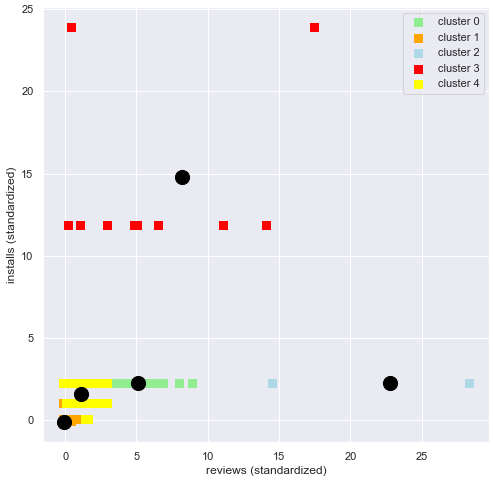
\includegraphics[scale=0.65]{kmeans6} \\ 

We can conclude that K=5 works well for the data. The black points are the cluster centroids. The red cluster are those apps with higher number of installs compared to reviews. The blue cluster are those apps with higher number of reviews compared to installs. One of the weaknesses of K-means is it's sensitive to outliers. I did not remove any outlier points for this scenario.
\end{document}




